\chapter{Particle and Event Reconstruction}
\label{chap:reco}

After the digitization step, each event is a collection of hits in the
various sub-detectors. In order to extract physically meaningful
quantities from these hits, a set of algorithms has been developed to 
efficiently reconstruct the stable particles produced by a
collision. In the following chapter, the various reconstruction
algorithms will be discussed along with the physical particles to
which they are associated. 

\section{Inner Detector Tracks}
\label{chap:reco:sec:tracks}

Interesting scattering processes nearly always include charged
particles in the final state. The two tracking systematics in ATLAS, the ID and the muon
system, are designed to measure the trajectories of these charged
particles, from which momentum 4-vectors are derived. A track is fully
specified by five parameters $\vect{\alpha} = ()$. In the following section,
the algorithms for fitting these parameters from detector hits will be
described. 

\subsection{Inside-out Tracks}

The primary tracking algorithm in ATLAS builds tracks starting with
hits in the pixel detectors, and progressively adding hits at larger
$r$ values. This is known as the inside-out track reconstruction
paradigm~\cite{bib:Cornelissen:2007vba}. Starting with hits from the pixel and SCT detectors,
collectively known as the silicon detectors, clusters of contiguous
hits are identified and associated with a coordinate in space. The
track-finding algorithm is seeded by a group of three clusters in
different layers that is consistent with a track. This seed defines a
``road'' along which the track candidate is built. The track
trajectory is propagated through the detector in a Kalman filter based
approach~\cite{bib:Fruhwirth:1987fm}. At the $k^{\textrm{th}}$ detector layer, the hit
that is most consistent with the track parameters from the previous
layer is assigned to the track. The track parameter vector is then
updated with the new hit included, yielding $\vect{\alpha}_k$. The propagation to the subsequent
layer is then given by

\begin{equation}
\vect{\alpha}_{k+1} = M_k\vect{\alpha}_{k} + \vect{\epsilon}_{k}
\end{equation}

\noindent
where $M_k$ is the linear map representing the magnetic field between the
two detector layers, and $\epsilon_{k}$ is a stochastic term that
accounts for multiple scattering of the charged particle. The
procedure is then repeated at layer $k+1$. The above approach for
fitting the track parameter vector is equivalent to a global minimum
least-squares fit. 

After all of the seeds have been evaluated by the Kalman-filter
algorithm, ambiguities are removed from the resulting track candidate
collection. These ambiguities include track candidates that share one
or more hits, are incomplete, or include hits that arise from more
than one charged particle. In order to resolve these ambiguities, the
tracks are first refitted using a detector geometry with a more
realistic description of the detector material. Each track is then
assigned a score that quantifies the quality of the track. Tracks with
more hits receive higher scores, and these scores are weighted
according to the precision of the detector subsystem in which the hit
reside. Given the high intrinsic efficiencies of the silicon
detectors, if a hit is absent along a track trajectory, the track
score is penalized. After track scoring, hits that are shared by more
than one track are assigned to the track with higher score. The
remaining track is then refitted and re-scored. Tracks that fail to
pass a score threshold are discarded.

The silicon only track candidates that pass the quality threshold are
the seeds for the extension of the track into the TRT. In
the first pass, the silicon hits that define the track seed for the
TRT extension are not changed. Again, the Kalman filter approach is
used to map the track from one detector surface to another. Along the
trajectory, TRT hits are added depending on the distance between the
Kalman filter prediction and the actual hit location. With the TRT hits
identified, the track is refitted with the hits from all
subdetectors-- silicon and TRT. In this pass, the silicon hits are
allowed to vary. The score of the refitted track is compared to that of
the silicon only track, and if it is smaller, the silicon only track
is retained, with the hits from the TRT as outliers, but still
associated to the track. If the score of the refitted track is larger,
this new track is retained. 

\subsection{Outside-in Tracks}

Because the inside-out algorithm is seeded by silicon clusters
associated to a primary vertex, it fails to find tracks arising from
secondary decays that occur late in the silicon system or in the
TRT. These tracks include those associated with electrons
from photon conversions and charged hadrons or leptons from hadron
decays. To recover secondary tracks, an outside-in algorithm, starting
in the TRT, is used in concert with the inside-out algorithm. 

Since TRT hits do not have information about the global $z$
coordinate in the barrel, it is not possible to use pattern-finding
procedure based on three-dimensional space coordinates as is done in
inside-out tracking. Instead, the TRT hits are projected to the
$r-\phi$ plane in which they form straight lines. The hits are then Hough
transformed~\cite{bib:Duda:1972uht} to the parameter
space of a line, where the coordinate are the $y$-intercept, or the
initial $\phi$ of the line, and the slope, or $1/p_{\textrm{track}}$,
where $p_{\textrm{track}}$ is the momentum of the track. In this
space, track candidates appear as maxima at their respective
($\phi_0,1/p_{\textrm{track}}$) coordinates. This technique, which
defines the hit $r-\phi$ coordinate to be the center of the straw,
fails to incorporate information about the drift time. In a second
step, the track candidates are refitted with a Kalman-filter-based
algorithm that incorporates information about the drift time, thereby
improving the accuracy of the fitted track parameters. 

The final step of the outside-in track reconstruction algorithm is the
extension of the TRT segments into the silicon tracker (need good
reference for this). Scanning longitudinally in a small $r-\phi$ wedge
defined by the TRT segment, the algorithm searches for at least two
clusters of SCT hits in the three outmost layers of the
SCT. Once found, the curvature defined by these two three-dimensional
points and the first TRT hit in the TRT segment is computed, and if
the result is unreasonable, the two clusters are disregarded. The SCT
clusters that are retained seed the track-fitting algorithm,
propagating the track to smaller $r$ and extracting the fitted track
parameters. 

\subsection{Vertex Reconstruction}



\section{Calorimeter Clustering}
\label{chap:reco:sec:cluster}

The ATLAS calorimeter system, described in section~\ref{chap:lhc_atlas:sec:calorimeter}, is crucial
for reconstructing electrons, photons, jets, and missing transverse
energy. Just as tracks are reconstructed from hits in the ID,
calorimeter cells are grouped into clusters that represent the
transverse energy of incident particles. With the energy and direction
information from the clusters, it is possible to reconstruct the
4-momentum of a particle. Moreover, cluster shapes are used to identify
the particles in the collision. Two types of clustering algorithms are
used in ATLAS: sliding window and topological clustering~\cite{bib:Lampl:2008zz}. The former
is effective in the reconstruction of electrons, photons, and hadronic
$\tau$ decays, while the latter is most performant for jets and
missing transverse energy.

\subsection{Sliding window clustering}
\label{chap:reconstruction:sec:cluster:subsec:sliding_window}

In sliding window clustering, calorimeter cells in a fixed rectangular
$\eta-\phi$ window are summed, and clusters are built around windows
for which \et~is maximized. The first step is to partition the
calorimeter into an $\eta-\phi$ grid with each grid element having dimension
$\Delta{\eta}\times \Delta{\phi} = 0.025 \times 0.025$. For each grid
element, the enclosed cell energies are summed across the calorimeter layers,
yielding a ``tower'', the object from which clusters are
constructed. A window of area $\eta_{\textrm{window}} \times
\phi_{\textrm{window}}$ is scanned across the grid of towers, and at
each point, the transverse energy sum of all towers within the window
is computed. If a local maximum above an energy threshold is found, the location associated with
this point is computed as the weighted vector sum of the tower
energies, and the resulting $(\eta,\phi)$ coordinate is used to seed the final step in which the
clusters are built. If two of these seeds fall within two $\eta$ or
two $\phi$ grid units of eachother, the seed with the lower \et~is
discarded. 

Calorimeter cells are assigned to a cluster if they are enclosed by the
rectangle of size $\eta_{\textrm{cluster}} \times
\phi_{\textrm{cluster}}$ centered at the seed defined in the previous
step. The dimensions of the cluster rectangle as well as the seed
location depend on the calorimeter layer. Furthermore,
$\eta_{\textrm{cluster}}$ and $\phi_{\textrm{cluster}}$ vary depending on
the predicted particle type. In the barrel region, the window size for electrons and
converted photons is $3 \times 7$ in units of $\Delta{\eta}\times
\Delta{\phi}$. Because electrons bend in the $\phi$ direction in the ID
$B$-field and emit {\it Bremsstrahlung} photons, electron calorimeter
showers tend to be elongated in the $\phi$ direction. Similarly,
photons that convert to electron-positron pairs also have showers that
are elongated in $\phi$, and therefore the window is set to $3 \times
7$. Unconverted photons, on the other hand, tend to shower in a
smaller $\phi$ region, and consequently the window dimension is $3
\times 5$. 

\subsection{Topological clustering}
\label{chap:reconstruction:sec:cluster:subsec:topo}

In contrast to sliding window clustering, the topological clustering
algorithm iteratively adds neighboring cells to seed cells, resulting in variable
size clusters. Seed cells are calorimeter cells with a signal-to-noise
ratio that falls above a large threshold $t_{\textrm{seed}}$. Signal
is defined as the energy deposited in the cell for the EM calorimeter,
and as the absolute value of the energy in the hadronic
calorimeter. There are two sources of noise: readout electronics and
pileup. Noise from the electronics is computed based on the cell
gain, while the expected noise to due pileup is estimated from the
beam conditions, and the two components are added in quadrature. The
noise in hadronic calorimeter cells in the outermost barrel layer as a
function of the mean number of interactions per bunch crossing is
shown in figure~\ref{chap:reconstruction:fig:tile_noise}. In these
cells, the pileup noise increases fairly linearly with $\left \langle \mu \right \rangle$.

\begin{figure}[h]
    \centering
    \includegraphics[width=0.6\textwidth]{fig/reconstruction/noise_D5D6_8TeV_25ns_newLVPS.eps}
    \caption[]{Noise in hadronic calorimeter cells located in the
    outermost layer in $0.9 < |\eta| < 1.3$ as a function of
    $\left \langle \mu \right \rangle$. Collision data at $\rts = 7 \tev$ with 25 ns bunch spacing
    is shown in blue and red. Data points at $\left \langle \mu \right \rangle > 20$ are from
    simulation. The dashed line is the expected noise from
    electronics.\cite{bib:Araque:1561207}}
\label{chap:reconstruction:fig:tile_noise}
\end{figure}

Seed cells, called proto-clusters, are ranked according to $S/N$ and for
each seed, if a neighboring cell passes another $S/N$ threshold,
$t_{\textrm{neighbor}}$, the neighbor is added to the
proto-cluster. In cases where the neighboring cell is adjacent to two
nearby seeds, the two proto-clusters are merged. In the next
iteration, the neighbors with $S/N > t_{\textrm{neighbor}}$ become the
new seeds, and the procedure is repeated. Neighboring cells
which pass a threshold $t_{\textrm{cell}}$, but fall below
$t_{\textrm{neighbor}}$, are added to the proto-cluster, but do not
become seeds in the subsequent iteration. These low $S/N$ cells are
retained to better model the tails of the calorimeter shower. Cluster
building continues until the list of seeds is exhausted. Because
neighboring cells include those in adjacent calorimeter layers in
addition to those in the $\eta-\phi$ plane, the
resulting topological clusters are three-dimensional objects which
can span across the EM and hadronic calorimeters. 

For events with low particle multiplicity, the clustering algorithm
described above is sufficient. However, due to the high energy density
of actual ATLAS events, the above algorithm creates clusters
that span large regions of the calorimeter. To resolve individual
particles, the clusters are split into sub-clusters, using local energy
maxima within the clusters. If a cell has $E > 400$~\mev, this energy
is greater than that of the neighboring cells, and four or more
neighbors have $S/N$ above a threshold, the cell is added to a list of
seeds. These seeds are then used to grow clusters with the same
algorithm in the previous step, except that only the cells that fall
within the parent cluster are added, no threshold is applied, and
overlapping clusters are not merged, i.e. cells can be associated with
two clusters, and the energy of the cell is shared between the two
clusters. The resulting collection of clusters is combined with
the parent clusters without local maxima to form the final list of
topological clusters in the event. 

There are two topological cluster types in ATLAS, defined by
the $S/N$ thresholds for cluster building. The ``electromagnetic 633''
(``combined 420'') cluster type has $t_{\textrm{seed}}=6~(4)$,
$t_{\textrm{neighbor}}=3~(2)$, and $t_{\textrm{seed}}=3~(0)$. Electromagnetic
633 clusters only use cells from the EM calorimeter, while combined
420 clusters can include cells from either calorimeter. With higher
$S/N$ thresholds, the rate at which noise results in a cluster is
smaller for EM 633 clusters. Combined 420 clusters, on the other hand,
have been optimized to find low energy deposits, with sufficient noise
rejection power. 


\section{Electrons}
\label{chap:reco:sec:electron}

\subsection{Electron reconstruction}

Electrons and photons appear in many interesting final states,
including Higgs decay chains, making it crucial to efficiently
reconstruct these particles. In the ATLAS detector, an electron is
loosely defined as energy deposits in the EM calorimeter matched to a
reconstructed track. Sliding window clustering, described in
section~\ref{chap:reconstruction:sec:cluster:subsec:sliding_window},
is used. The efficiency for finding the EM showers associated with a
true electron with sliding window clustering is 95\% at $\et =
7~\gev$, increasing to 99.9\% at $\et =
45~\gev$~\cite{bib:ATLAS-CONF-2014-032}.

Tracks associated with electron candidates are reconstructed with the
algorithms discussed in section~\ref{chap:reco:sec:tracks}, with some
important differences to account for the propensity for electrons to
emit radiation as they pass through matter. Electron track candidates are extended
through the inner detector with the Kalman filter approach. In the
first fit attempt, scattering in the detector material assumes the
particle is a pion. Upon reaching the calorimeter, if the track does
not overlap with a region of interest (ROI), defined as the $\Delta{R}
< 0.3$ region around the center of an EM cluster which satisfies loose
shower shape requirements, then starting from the
track seed, the track is propagated again, instead assuming an
electron-like interaction with the detector material. The electron
hypothesis allows for up to 30\% energy loss due to {\it
  Bremsstrahlung}. All track candidates found to overlap with ROIs are
then re-fitted using the global $\chi^2$ track-fitting algorithm. These
tracks are extrapolated to the middle layer of the EM calorimeter. For
each of these track candidates, one of two requirements must be satisfied:
(1) the track falls within $\phi = 0.2$ in the direction of deflection
and $\phi = 0.05$ in the opposite direction, and within $\eta = 0.05$
of the center of the EM cluster, (2) after rescaling the track
momentum by the measured cluster energy, the track is within $\phi =
0.1$ in the direction of deflection and $\phi = 0.05$ in the other
direction of the center of the EM cluster. These two requirements are
adjusted slightly for track candidates with less than 4 silicon
hits (TRT-only tracks). Requirement (2) is designed to retain low \pt~tracks that may
have suffered significant energy losses before reaching the
calorimeter.

With the exception of TRT-only tracks, tracks that pass either of the requirements are then re-fitted again
with the Gaussian Sum Filter (GSF)
algorithm~\cite{bib:ATLAS-CONF-2012-047}, which is a generalization of
the Kalman filter algorithm that accounts for nonlinear effects from
{\it Bremsstrahlung}. The re-fitted
tracks are matched to EM clusters again, this time with tighter
requirements on the $\Delta{\phi}$ and $\Delta{\eta}$ distances. For
cases in which more than one track is associated to a cluster, tracks
with more pixel hits that fall closer to the cluster center are
favored. 

With tracks matched to clusters, the calorimeter clusters are then
rebuilt in each layer using sliding window dimensions that have been
optimized for electrons. The size of the window is $3 \times 7$ ($5
\times 5$) in the barrel (endcaps). In order to reduce the
uncertainties on the measured energy, a multivariate regression
technique is used to correct for instrumental effects. The regressor,
which has been trained on single electron events, determines a
correction factor for the total cluster energy, using as independent
variables the total energy measured in the calorimeter, the ratio of
the presampler energy to the EM calorimeter energy, the shower depth,
the pseudorapidity of the center of the cluster in the global
coordinate system, and the $\eta$ and $\phi$ of the cluster in the
calorimeter coordinate system~\cite{bib:Aad:2014nim}. The performance
of the MVA technique is summarized in
figure~\ref{chap:reconstruction:fig:elec_mva}. The most
probable value (MPV) of the ratio of the measured energy to the true
energy as a function of $\eta_{\textrm{electron}}$, an
estimate of the linearity of the technique, is less than 0.5\% across
the \et~range in the barrel region, while in the forward calorimeter
the effect is slightly larger due to more detector material in front
of the calorimeter. Similarly, the relative energy resolution ($\sigma/E$) grows
with $|\eta|$ due to material effects. 

\begin{figure}[ht]
    \centering
    \subfigure{
    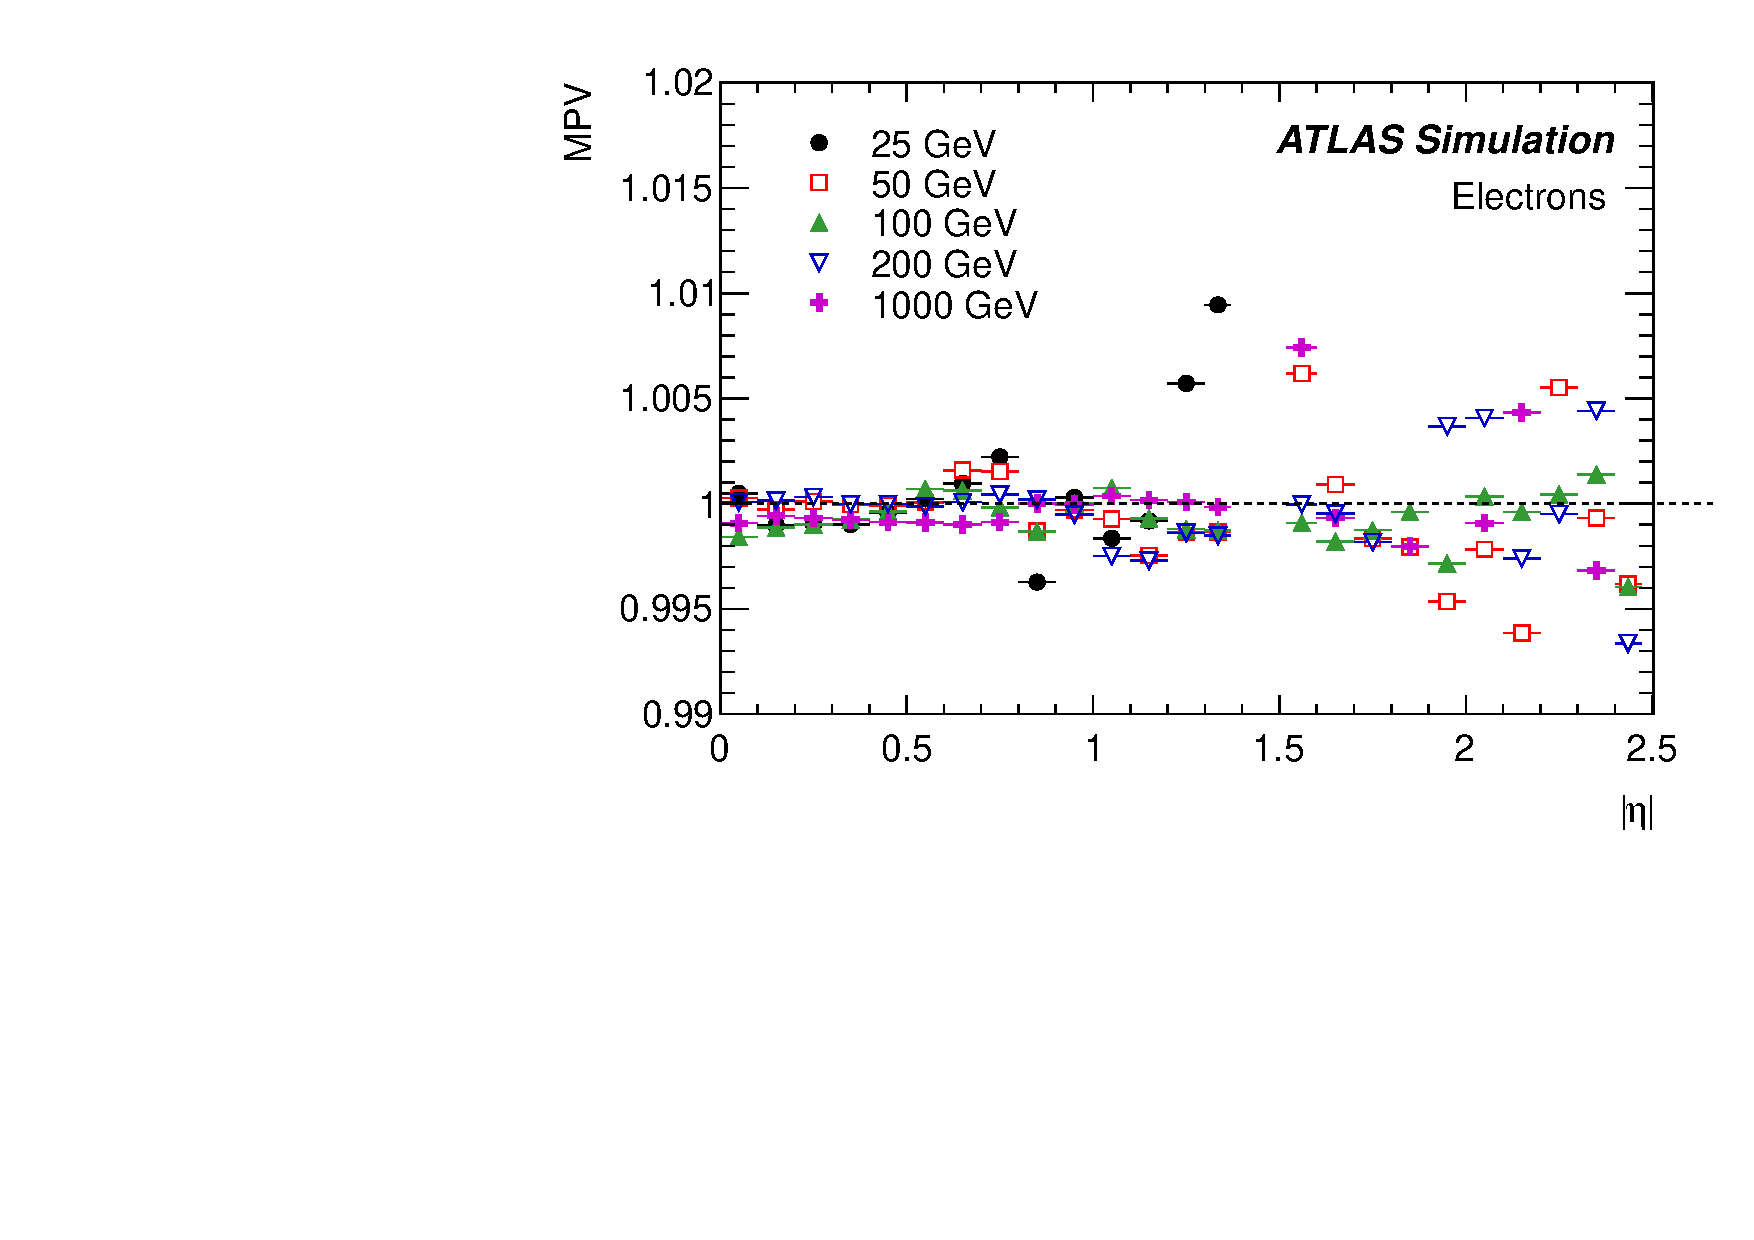
\includegraphics[width=0.4\textwidth]{fig/reconstruction/elec_mva_EdivEtrue.pdf}
    \label{chap:reconstruction:fig:elec_mva_EdivEtrue}
    }
    \subfigure{
    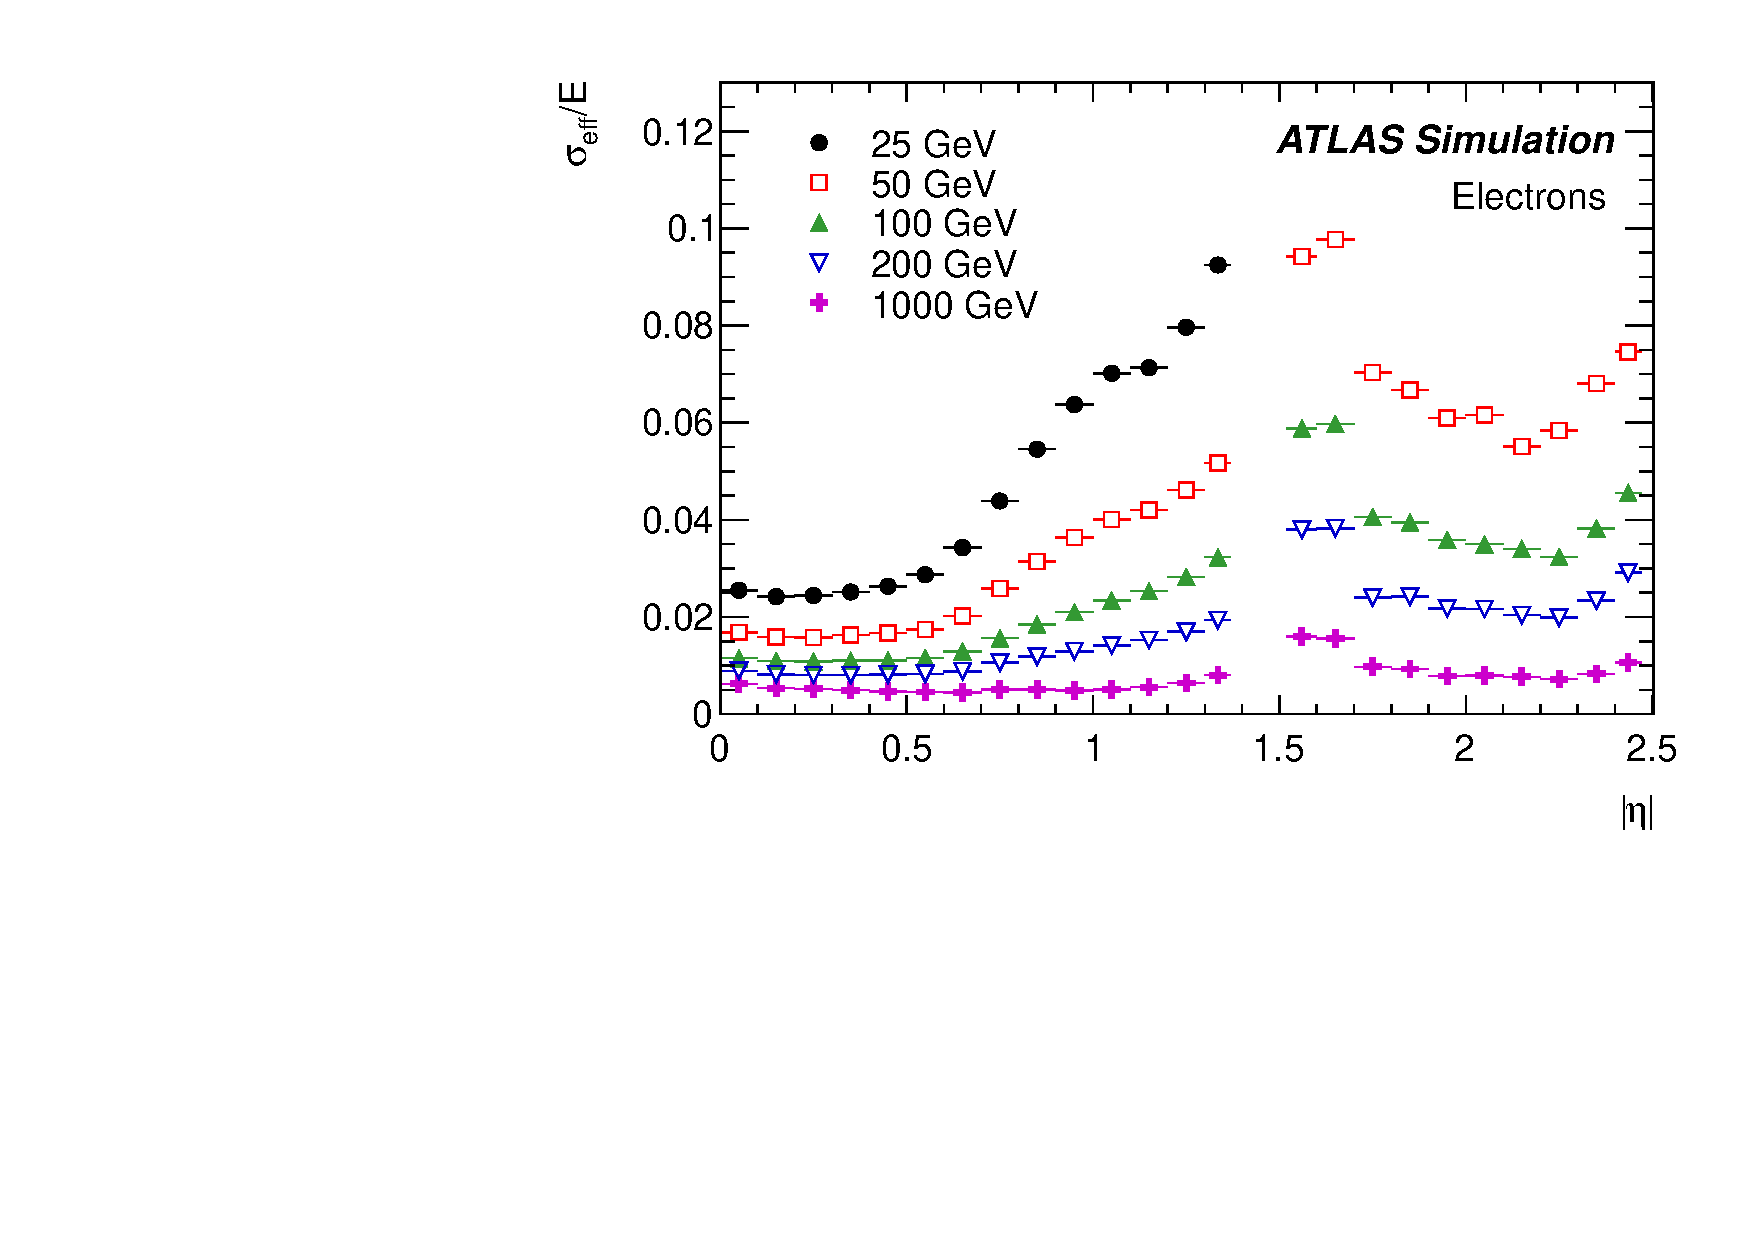
\includegraphics[width=0.4\textwidth]{fig/reconstruction/elec_mva_resolution.pdf}
    \label{chap:reconstruction:fig:elec_mva_resolution}
    }
    \caption[]{The most-probable-value (MPV) of the ratio of the
      measured energy to the true
      energy~\subref{chap:reconstruction:fig:elec_mva_EdivEtrue} and
      the energy
      resolution~\subref{chap:reconstruction:fig:elec_mva_resolution}
      as a function of $\eta_{\textrm{electron}}$ for electrons of
      various \pt.~\cite{bib:Aad:2014nim}}
\label{chap:reconstruction:fig:elec_mva}
\end{figure}

The 4-momentum of the reconstructed electron candidate is derived from
both calorimeter and track information. The electron energy is taken
from the calorimeter cluster, while the $\eta$ and $\phi$ are taken from
the best-matched track. For TRT-only tracks, $\eta$ and $\phi$ from
the cluster are used. 

\subsection{Electron identification}

Electrons which are reconstructed according to the algorithm described
in the previous section can arise from backgrounds, including charged
hadrons, semi-leptonic heavy flavor hadron decays, the Dalitz decay of the pion ($\pi_0
\rightarrow{e^+ e^- \gamma}$), and photon conversions. To suppress
these backgrounds while retaining true prompt electrons, candidates are
identified using a collection of discriminating variables, either
placing sequential cuts on the variables, or using them as inputs to a
multivariate algorithm. In the tracking region ($\eta < 2.47$), signal
and background electrons are distinguished by variables which describe the
EM shower shapes, properties of tracks, as well as the
matching between the track and EM cluster~\cite{bib:ATLAS-CONF-2014-032}. 

Cut-based electron identification cut criteria are categorized based
on the rejection power. In order of increasing rejection-- and decreasing
efficiency-- the categories are called {\it loose}, {\it medium}, and
{\it tight}. Electrons selected with the {\it tight} criteria are a
subset of {\it loose} and {\it medium}, and those selected with {\it
  medium} are a subset of {\it loose}. These selection criteria have
been optimized in bins of electron \et~and $\eta$ to account for the
fact that shower shapes vary with these quantities. 

To improve on the cut-based identification approach, the same
discriminating variables are used in a likelihood-based multivariate
technique. The electron likelihood is defined by the equation

\begin{equation}
L_{s(b)}(\vect{x}) = \prod_{i=1}^n P_{s(b),i}(x_i)
\end{equation}

\noindent
where $P_{s(b),i}(x_i)$ is the signal (background) probability
density function (p.d.f.) for the $i^{\textrm{th}}$ variable evaluated at
$x_i$. The p.d.f.s are obtained from data in control regions. Track
hit requirements are not included in the likelihood and are instead
left as cuts. As in cut-based electron identification, there are three
selection categories based on background rejection. The
\textsc{loose}, \textsc{medium}, and \textsc{very tight} categories
correspond to different cuts on the likelihood-based discriminant
$L_s/(L_s+L_b)$, and the cut values are chosen such that the
efficiencies are approximately the same those of the corresponding
cut-based categories. In addition to different discriminant
cut-values, each likelihood category uses a different set of input
variables in the likelihood. The \textsc{loose} category features
variables that are efficient in rejecting electron candidates in
light-flavor jets, while \textsc{medium} and \textsc{very tight}
include additional variables that help in the discrimination against
heavy flavor jets and photon conversions. The p.d.f.s that define the
likelihood are subdivided into nine $|\eta|$ bins and six \et~bins
whose boundaries roughly correspond to those in cut-based
identification. Due to limited data statistics, however, the binning
is coarser for likelihood-based electron identification.

In addition to the identification requirements above, hadronic
backgrounds are further rejected by requiring that the electron
candidates are isolated. Two types of isolation cuts are
applied. Calorimeter-based isolation requires that the sum of the
transverse energy in a $\eta-\phi$ radius around the electron is less
than some value. Similarly, track-based isolation requires that the
sum of the \pt~of tracks with $\pt>4 \gev$ in a $\eta-\phi$ radius
around the electron is small. The specific isolation cuts used in the analysis
presented in this thesis are discussed in section~\ref{}

%\begin{table}[h]
%  \centering
%  \begin{tabular}{llrr}
%  \hline
%  
%  \end{tabular}
%  \caption[MC sample summary.]{MC sample summary with corresponding
%  cross sections.}
%  \label{chap:analysis:tab:mc_summary}
%\end{table}

Understanding the efficiency-- and associated uncertainties-- for
selecting an electron is crucial to all ATLAS analyses with electrons
in the final state. In order to measure the efficiencies, a sample of
true electrons is needed. This can be obtained by using the truth
record in MC simulation, whereby a true electron is matched to a
reconstructed electron, and the fraction of reconstructed electrons in
the sample of true electrons is extracted. However, due to the strong dependence on the
material model in the simulation, the electron efficiency measurements
use ATLAS data in phase space regions where true electrons are
likely to reside. 

Electron efficiencies are measured with a data-driven technique called
``tag and probe''~\cite{bib:ATLAS-CONF-2014-032}. A tag electron is identified with {\it tight}
requirements, the remaining electron candidates in the events are
scanned over, and if the invariant mass of the electron pair falls
within $15 \gev$ of the $Z$ pole mass, the second electron is
considered a probe electron and put into a set called the
``denominator''. Because the invariant mass falls at the
$Z$ resonance, the probe electron is likely a true electron from the
$Z$ decay. Each electron in the denominator set is then required to
pass either a reconstruction or an identification condition, depending
on the efficiency being measured, and if a given electron passes, it
is placed in the ``numerator'' set. The ratio of the number of
electrons in the numerator to that of the denominator is the
efficiency, which is binned in electron \et~and $\eta$. 

The efficiency for selecting an electron can be factorized into four
components

\begin{equation}
\epsilon =
\epsilon_{\textrm{reco}}\cdot\epsilon_{\textrm{identification}}\cdot\epsilon_{\textrm{trigger}}\cdot\epsilon_{\textrm{additional}}.
\end{equation}

\noindent
The efficiency for reconstruction ($\epsilon_{\textrm{reco}}$) is
computed for electrons that pass the reconstruction algorithm
described in the previous section with respect to a denominator sample of EM
calorimeter deposits. The identification efficiency
($\epsilon_{\textrm{identification}}$) is computed for each
identification criteria, where the denominator sample is reconstructed
electrons with track quality cuts. The trigger efficiency is obtained
from electrons that have already been identified, and the final term is the
efficiency associated with isolation cuts or other electron quality
cuts. The latter two efficiencies, being dependent on analysis-level
cuts, will be discussed in chapter~\ref{chap:analysis}.

Tag-and-probe efficiencies for each identification category are
computed in bins of electron \et~and $\phi$. Tag-probe pairs are required to
fall in the $Z$ peak for $\et > 15 \gev$, while at lower \et,
\jpsi~decays are used. The numerator sample consists of probe electrons that
have passed a given identification criteria, while the denominator
sample is the superset of those electrons that have passed
reconstruction requirements and have one pixel hit and seven silicon
hits. Robust estimation of  backgrounds to \Zee~is critical for
avoiding biases in the efficiency measurements. To get the $M_{ee}$
shape template for backgrounds, identification cuts are inverted,
resulting in an orthogonal background rich sample. These templates are
then normalized using the high $M_{ee}$ sideband for the denominator,
and for the numerator sample, the region in which the electrons have
the same reconstructed charge is used to constrain the normalization. 

The tag-and-probe efficiencies for identifying electrons in each category are shown
in figure~\ref{chap:reconstruction:fig:elec_tp}, binned in
\et~\subref{chap:reconstruction:fig:elec_tp_et},
$\eta$~\subref{chap:reconstruction:fig:elec_tp_eta}, and the number of
primary vertices in the
event~\subref{chap:reconstruction:fig:elec_tp_npv}. Electron samples
have been obtained with $20.3~\ifb$ at $\rts = 8 \tev$. Efficiencies for
the cut-based categories agree with the associated likelihood
categories by design, with likelihood identification achieving better
background rejection. The efficiency increases with increasing \et~for
each of the categories with a value of \textapprox{95\%} (89\%) for
{\it loose} ({\it tight}) in the highest \et~bin. Features
in the $\eta$ distribution are well-understood. As the identification
criteria are tightened, isolated efficiency dips become more
pronounced. The dip at $\eta \sim 0$ is due to a small gap between the
calorimeter and the TRT, while the drop at $1.37 < |\eta| < 1.52$ is due
to the barrel-endcap transition in the calorimeter. Also, the drop at
high $|\eta|$ is due to the presence of more detector material in this
region. The electron reconstruction efficiency is fairly stable with
increasing pile-up, decreasing by a few percent as the number of
primary vertices increases. 

\begin{figure}[h!]
    \centering
    \subfigure{
    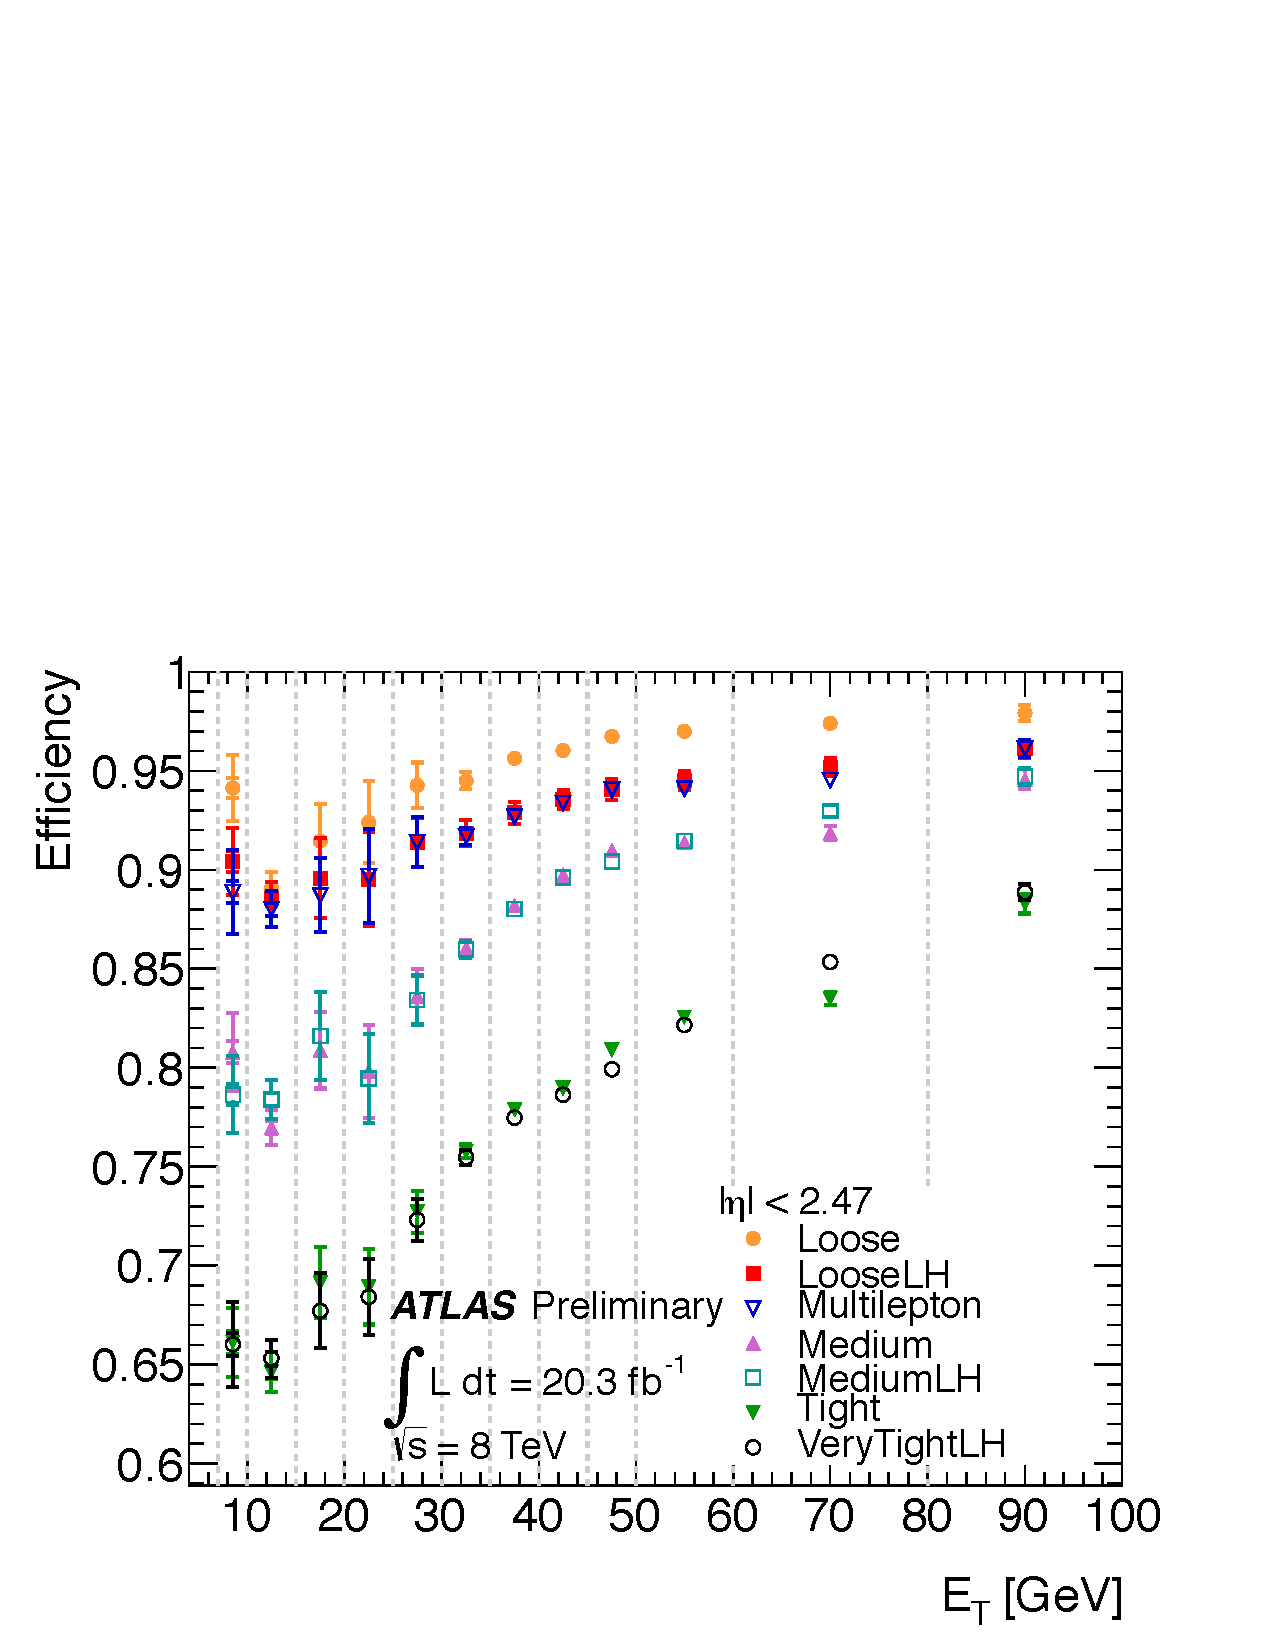
\includegraphics[width=0.4\textwidth]{fig/reconstruction/elec_TP_et.pdf}
    \label{chap:reconstruction:fig:elec_tp_et}
    }
    \subfigure{
    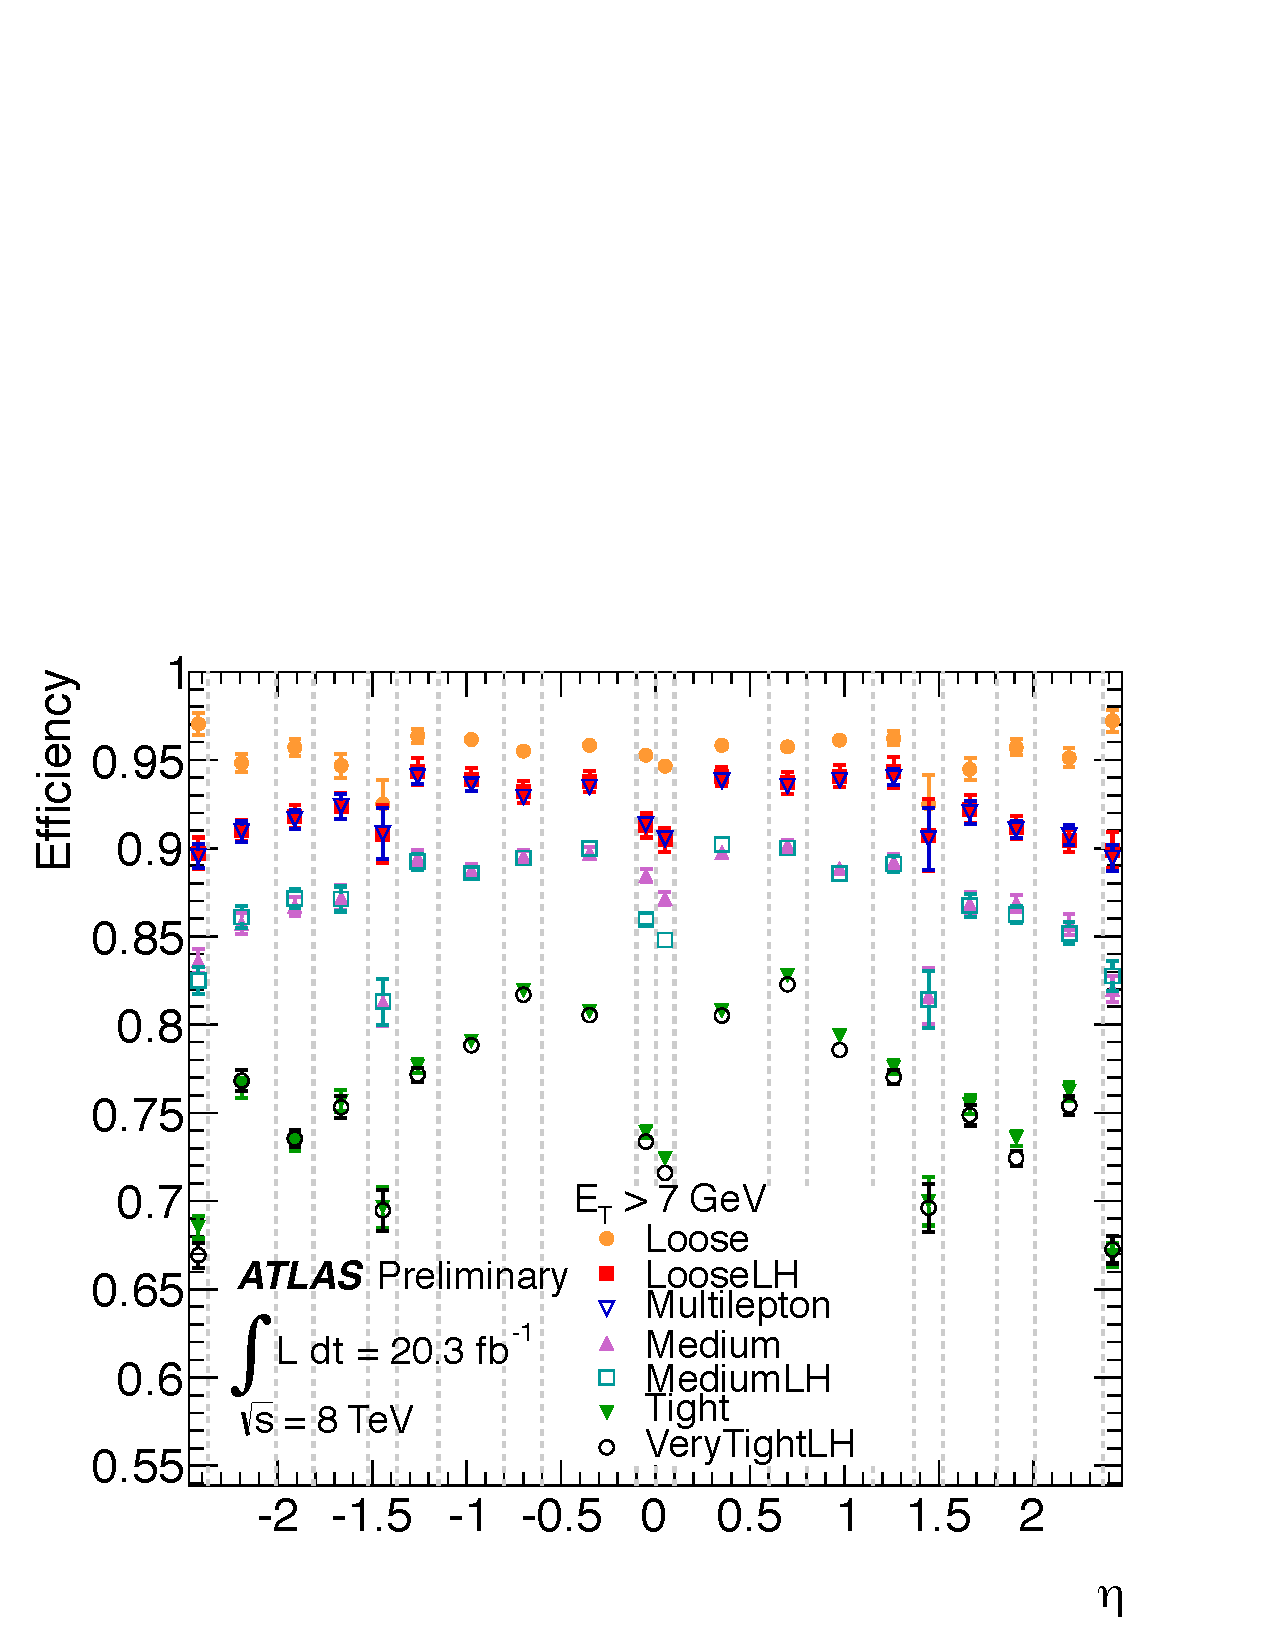
\includegraphics[width=0.4\textwidth]{fig/reconstruction/elec_TP_eta.pdf}
    \label{chap:reconstruction:fig:elec_tp_eta}
    }
    \subfigure{
    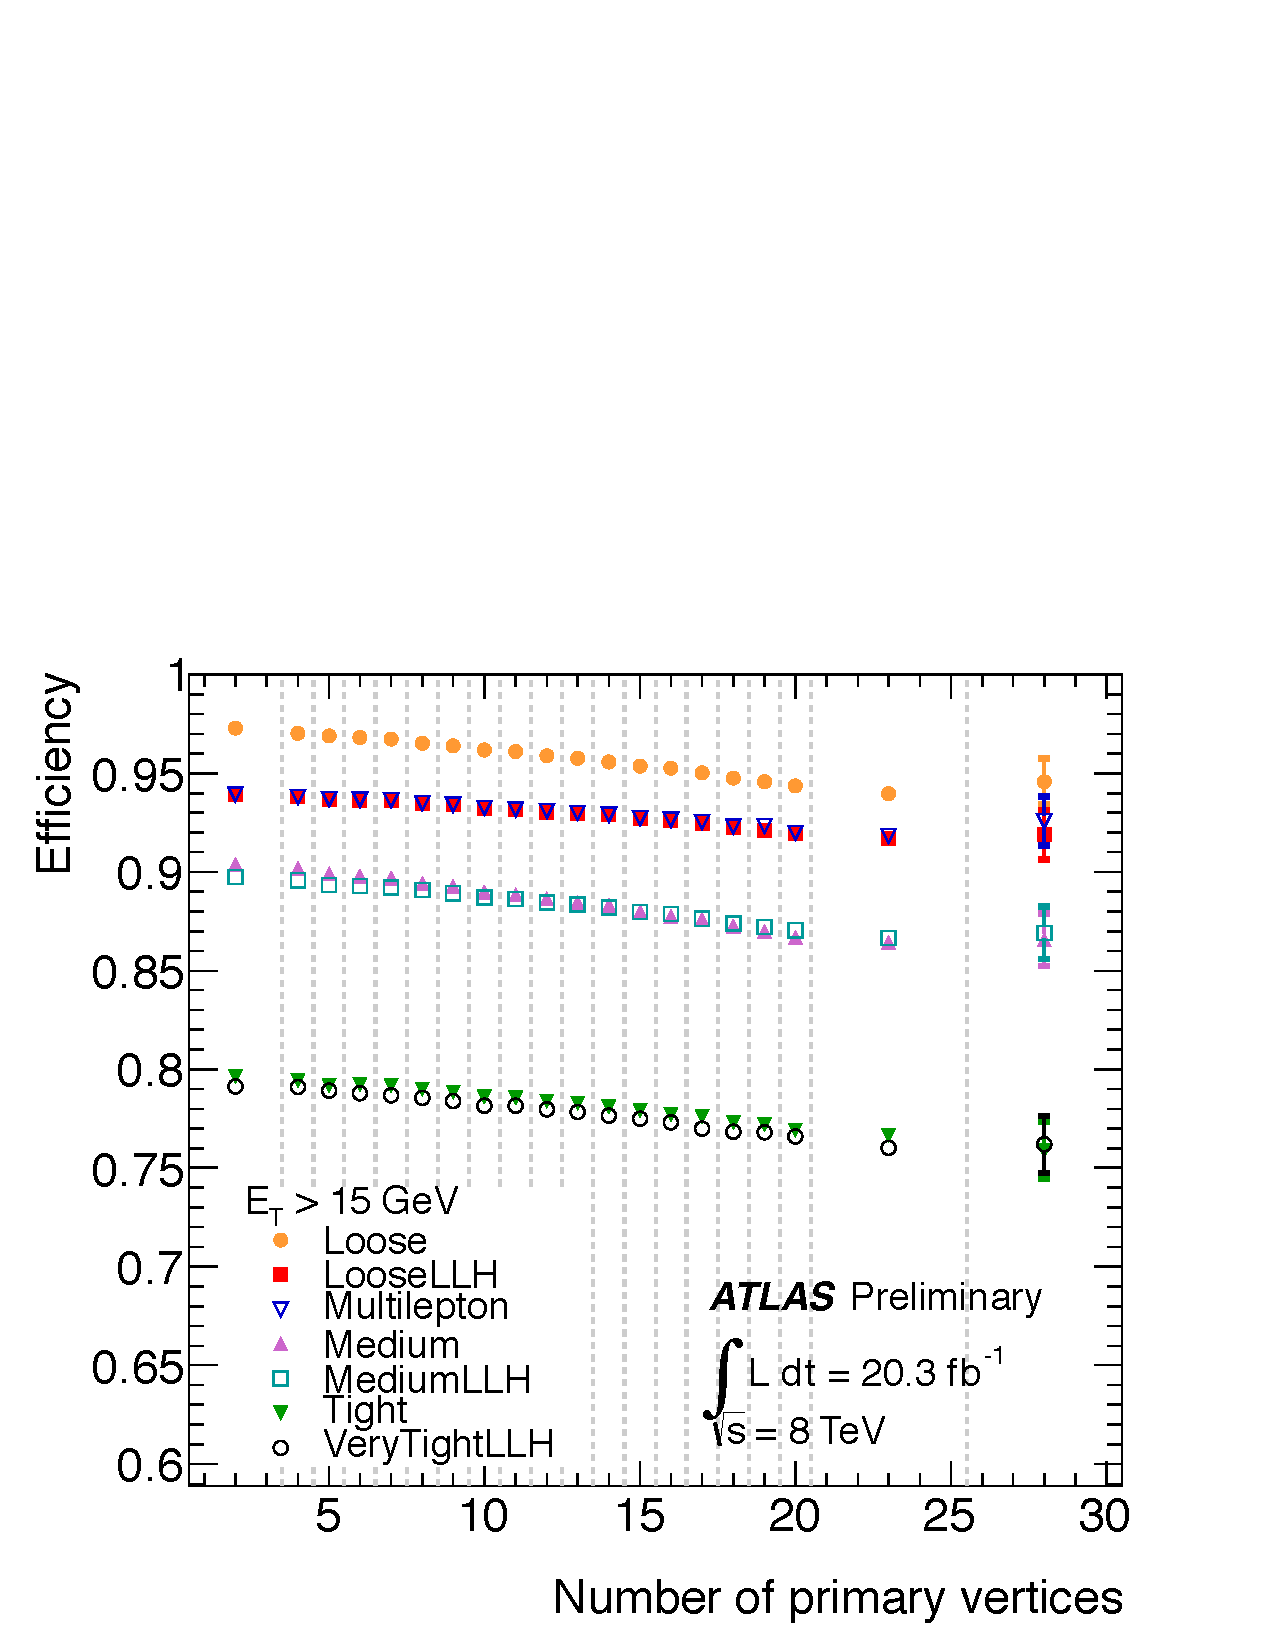
\includegraphics[width=0.4\textwidth]{fig/reconstruction/elec_TP_Npv.pdf}
    \label{chap:reconstruction:fig:elec_tp_npv}
    }
    \caption[]{Electron identification efficiencies for different
      cut-based and likelihood categories, binned in electron
      \et~\subref{chap:reconstruction:fig:elec_tp_et} and
      $\eta$~\subref{chap:reconstruction:fig:elec_tp_eta}, as well as
      the number of primary vertices in the
      event~\subref{chap:reconstruction:fig:elec_tp_npv}~\cite{bib:ATLAS-CONF-2014-032}.}
\label{chap:reconstruction:fig:elec_tp}
\end{figure}

The efficiency as measured in data is compared to simulated
\Zee~events. Tag and probe electrons are defined as they are in data,
but in the case of MC, the numerator set is the set of probe electrons
that fall within $\Delta{R} < 0.2$ of a true electron in the
simulation. The resulting efficiencies from MC are compared to those
of data, and the ratio of data to MC is computed as a correction which
is applied to MC. These ``scale factors'' are applied to each electron
identified in the event as a function of \et~and $\eta$.

In order to assess the uncertainties on the efficiency measurement--
and the associated scale factors-- several alternative measurements
are carried out. In addition to using the $Z$ peak to select
denominator electrons, a calorimeter isolation variable is used to
select denominator electrons and normalize the background
templates. Moreover, the width of the $Z$ mass window is varied, and the definition
of the tag electron is varied. In total, there are 90 systematic
variations on the efficiency measurement, with the central efficiency
set to the average and the systematic uncertainty the RMS. 


\section{Muons}
\label{chap:reco:sec:muon}

\subsection{Muon reconstruction}

Muons are reconstructed with information from the inner detector (ID),
the muon spectrometer (MS), and to a lesser extent, the
calorimeters. In the MS, track segments are first identified in each
layer, and then combined in a track fit (more information to be
consistent with other sections). Muon candidate tracks are
reconstructed in the ID according to the procedure in
section~\ref{chap:reco:sec:tracks}.

\subsection{Muon identification}

There are four muon identification schemes that take advantage of the
information from the different detector subsystems~\cite{bib:Aad:2014rra}. Stand-alone (SA)
muons are reconstructed with tracks from the MS only. The track of the
muon candidate is extrapolated back to the distance of closest
approach with the beam line, accounting for energy lost in the
calorimeter. These muons are required to have hits in at least two MS
layers. Because the MS extends to $|\eta| < 2.7$, SA muons recover
acceptance for muons which fall beyond the ID tracking volume $|\eta|
< 2.5$. For combined (CB) muons, muon tracks are independently
reconstructed in both the ID and the MS and then
combined. Segment-tagged (ST) muons are those for which there exists
an ID track which, when extrapolated to the MS, corresponds to a track
segment in a MDT or CSC layer. This type recovers acceptance
associated with muons that only traverse a single MS layer due to the
limited coverage of the MS or because the muon \pt~is low. Finally,
for calorimeter tagged (CaloTag) muons, an ID track is associated with
an energy deposit in the calorimeter that is consistent with a
minimum-ionizing particle. 

For the analysis presented in this thesis, only CB muons are used. The
combination of the ID and MS tracks is done by statistically combining
the two tracks with their respective parameters and covariance
matrices. Starting with a set of ID tracks and a set of MS tracks,
MS-ID track pairs are matched in $\eta$ and $\phi$, and the MS-ID track
pair with the smallest combined $\chi^2$ is retained as a CB muon. The
constituent tracks are then removed from the set and the next iteration
proceeds until there are no more candidate tracks. To suppress
background, the ID tracks that are used require at least 1 pixel hit,
5 SCT hits, and at least 9 TRT hits in the region with full TRT
coverage. Moreover, tracks can only have a maximum of 2 active pixel or
SCT sensors without hits along the track trajectory.

As with electrons, it is crucial to know the reconstruction and
identification efficiencies for muons of various transverse momentum
and pseudorapidity. The efficiencies are measured with the
tag-and-probe method on \Zmm~events in which two oppositely charged
and isolated muons with $\pt>25 (10) \gev$ have dilepton invariant
mass that falls within 10 \gev~of $m_Z$. Tag muons are required to
satisfy CB requirements, and the efficiency of identifying a probe CB
muon is measured as a function of \pt~and $\eta$, as shown in
figure~\ref{chap:reconstruction:fig:muon_tp}. The efficiency for CB
muons is between 95\% and 100\% across most of the $\eta$ range,
although it falls to zero at $|\eta|<0.1$, due to a gap in the MS
coverage. In general, the efficiency as measured in data agrees quite
well with that of simulation, with the exception of the barrel-endcap
transition region ($0.9<\eta<1.3$), where there are imperfections in the
modeling of the detector. (need to say something about the pT plot in
the figure).

\begin{figure}[h!]
    \centering
    \subfigure{
    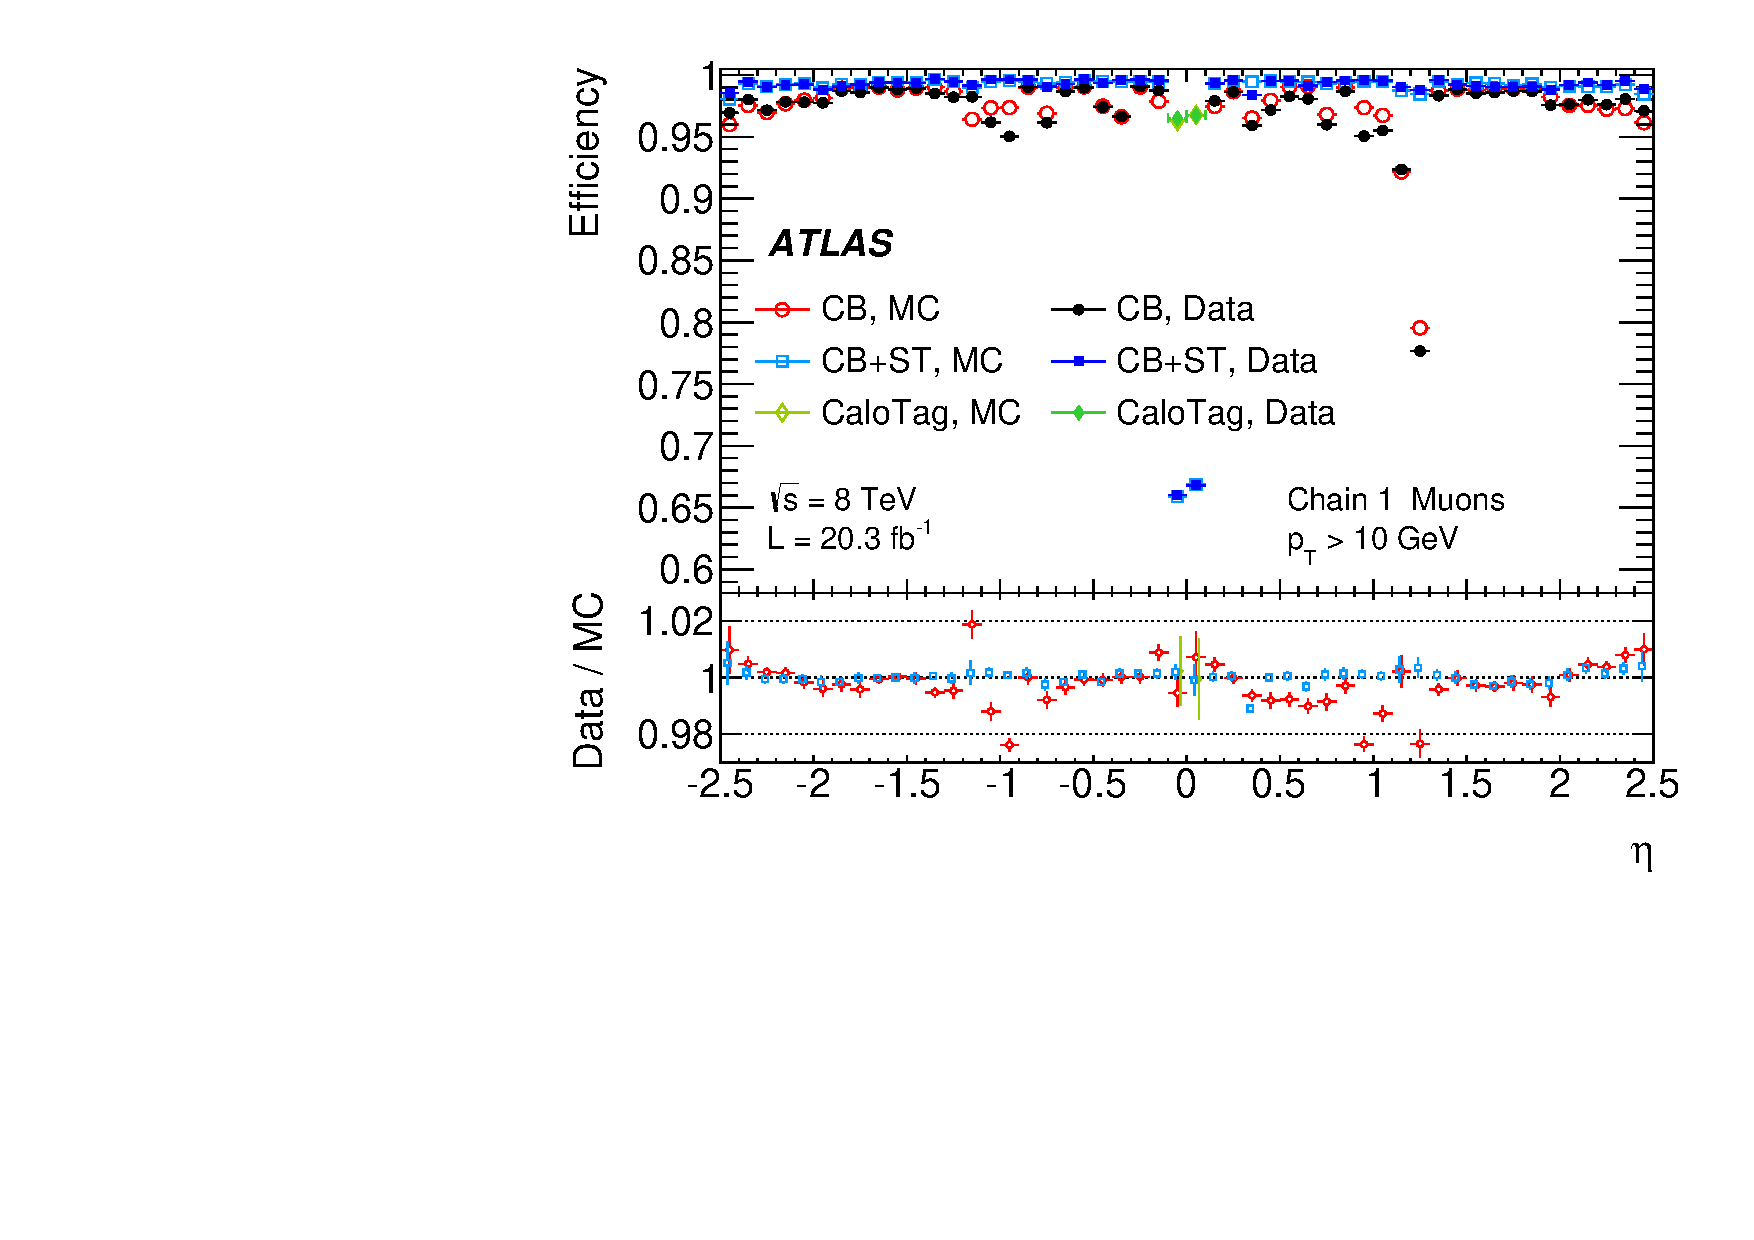
\includegraphics[width=0.4\textwidth]{fig/reconstruction/muon_TP_eta.pdf}
    \label{chap:reconstruction:fig:muon_tp_eta}
    }
    \subfigure{
    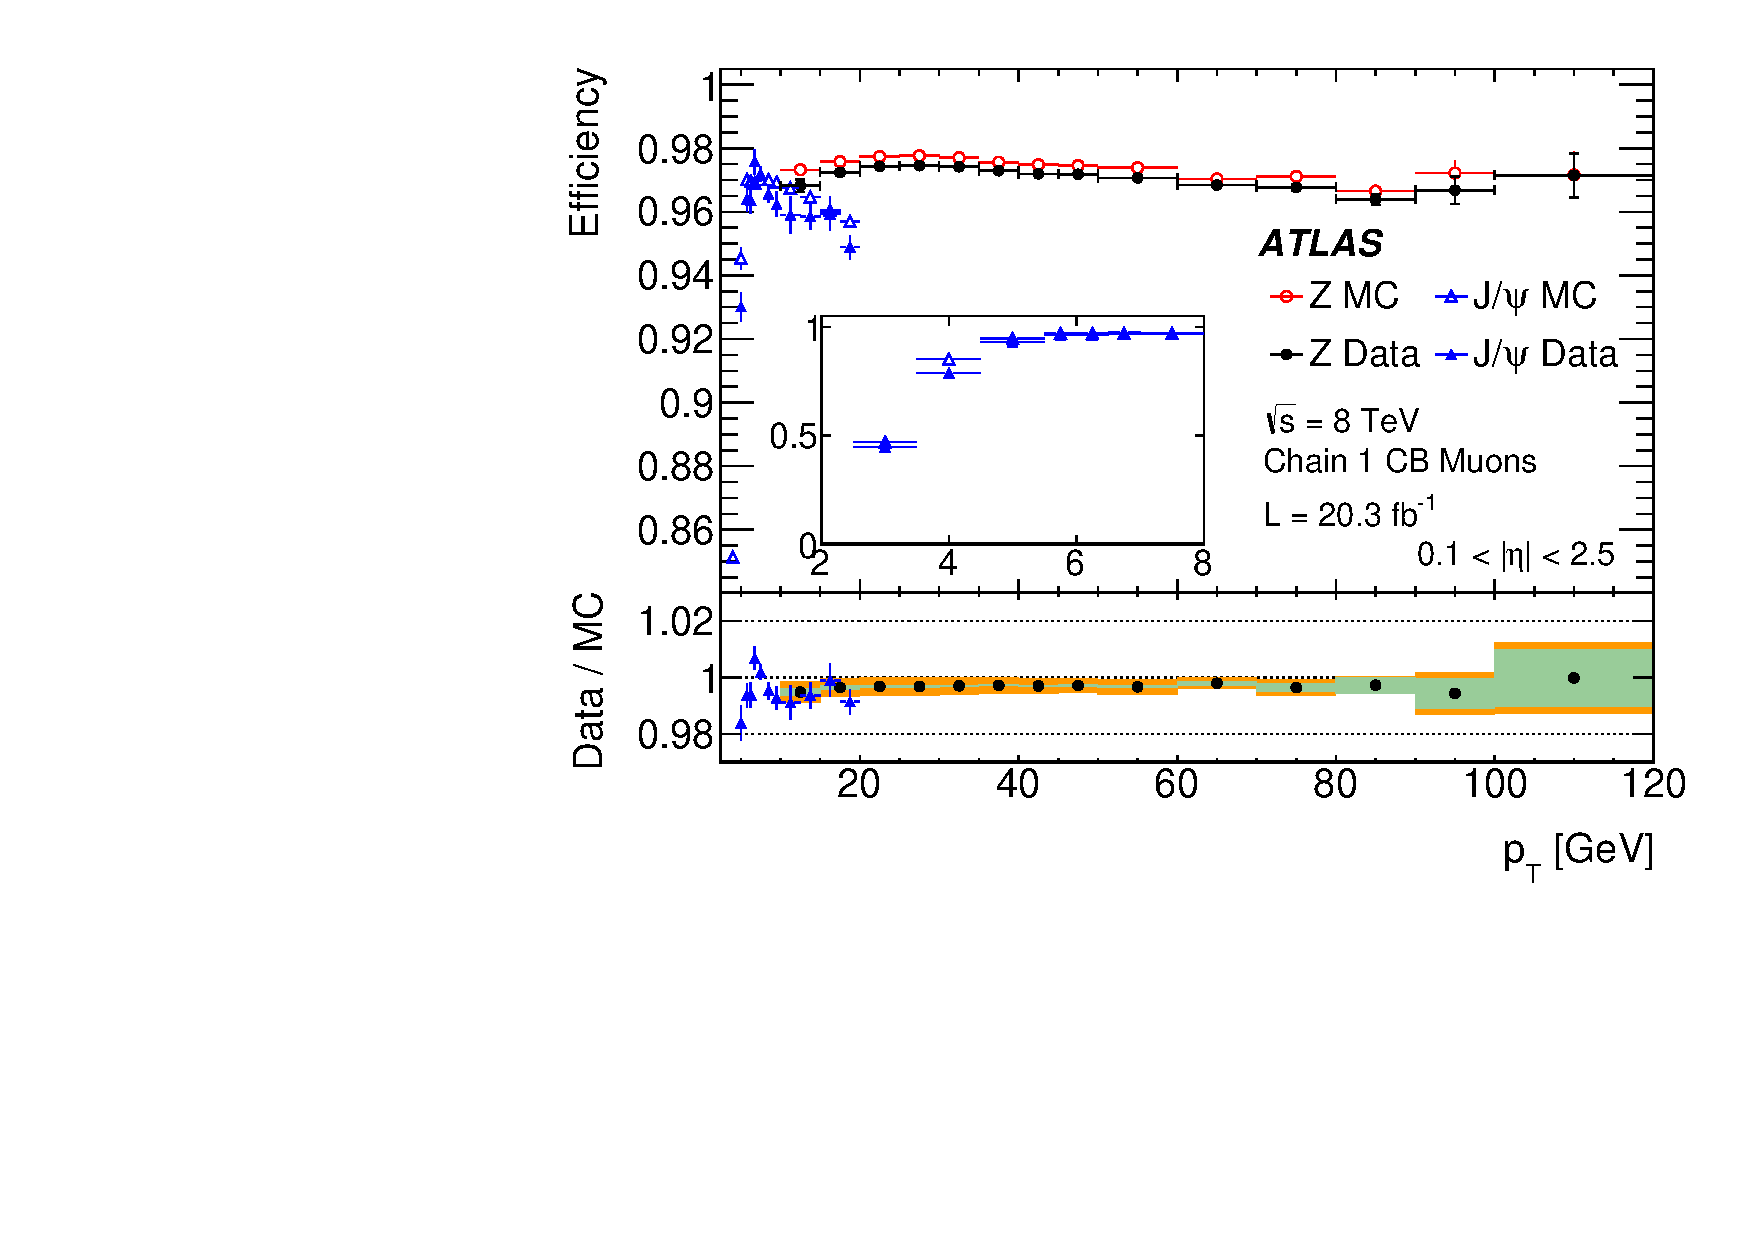
\includegraphics[width=0.4\textwidth]{fig/reconstruction/muon_TP_pt.pdf}
    \label{chap:reconstruction:fig:muon_tp_pt}
    }
    \caption[]{Muon identification efficiency as a function of
      $\eta$ for the different muon
      types~\subref{chap:reconstruction:fig:muon_tp_eta}, and as a
      function of \pt~for CB muons~\subref{chap:reconstruction:fig:muon_tp_pt}~\cite{bib:Aad:2014rra}.}
\label{chap:reconstruction:fig:muon_tp}
\end{figure}

As for electrons, the ratio of the efficiency measured in data to
simulation is computed. In order to recover the correct reconstruction
and identification efficiencies in simulation, these scale factors are
applied to all predictions from MC in two-dimensional $\eta-\phi$
bins. In addition to efficiency corrections, the muon momentum scale
and resolution is corrected in simulation, with corrections that are
determined in a likelihood fit to data. Scale corrections are less
than 0.1\% in most $\eta$ regions, and as high as 0.4\% in the region
$1.25 < \eta < 1.5$. Muon resolution is corrected in MC by applying a
``smearing'' term to the reconstructed \pt. This smearing correction is
less than 10\% for the ID and less than 15\% for the MS. Systematic
uncertainties on these corrections will be discussed in section~\ref{}.


\section{Jets}
\label{chap:reco:sec:jet}

A jet is loosely defined as a collection of collimated, high
\pt~hadrons arising as a result of the fragmentation and hadronization
of a parton or partons. Because partons do not exist as
observable particles, the constituent particles in jets-- which
manifest as tracks and calorimeter clusters-- must be combined in a
way that best reflects the parton 4-momentum. Jet algorithms are
designed to do this, while avoiding complications due to perturbative
QCD (pQCD). In pQCD, the probability for a quark to radiate a gluon
diverges in the soft ($E_{\textrm{gluon}}\rightarrow 0$) or collinear
  ($\Delta R_{\textrm{quark,gluon}}\rightarrow 0$) limits. Jet
  constituents are formed by a series of gluon emissions with
  subsequent quark splittings and are therefore difficult to model
  with pQCD. To ensure that the processes which form jets
  can be predicted with pQCD calculations, jet
  constituents are iteratively recombined until some condition
  that protects against infrared divergences is satisfied

\subsection{Anti-$k_t$ jets}

In ATLAS, jets are built with the \antikt
algorithm~\cite{bib:Cacciari:2008gp}. The jet constituents are the
topological clusters defined in
section~\ref{chap:reconstruction:sec:cluster:subsec:topo}. For each
event, starting with the full set of clusters, the quantity

\begin{equation}
d_{ij} = \min{(p_{ii}^{-2},p_{ij}^{-2})}\frac{\Delta{R_{ij}^2}}{R^2}
\label{chap:reconstruction:anti_kt}
\end{equation}

\noindent
is computed for each cluster pair. For the pair that yields the
minimum $d_{ij}$, if $d_{ij} < p_{ii}^{-2}$, the clusters are combined
and the next iteration begins with the new set of clusters. If the
above condition is not true, cluster $i$ is considered a ``jet'' and
is removed from the set of clusters. This process is repeated until no
more clusters exist. The parameter $R$ is called the distance
measure. If cluster $i$ has no clusters within $R$, then
$\frac{\Delta{R_{ij}^2}}{R^2} > 1$, making $p_{ii}^{-2}$ smaller than
$d_{ij}$, and the cluster is added to the list of
jets. Therefore, the distance measure controls the jet area and
protects against collinear divergences. To protect against soft
divergences, a minimum energy requirement is placed on the
clusters. The form of $d_{ij}$ in
equation~\ref{chap:reconstruction:anti_kt} is chosen to favor jets in
which soft clusters are grown around a hard ``seed'' cluster, due to
the $\min{(p_{ii}^{-2},p_{ij}^{-2})}$ term. In ATLAS, both $R=0.4$ and
$R=0.6$ jets are constructed with the implementation in
\fastjet~\cite{bib:Cacciari:2005hq,bib:Cacciari:2011ma}.

\subsection{Jet energy calibration}

Before combining calorimeter clusters with the \antikt algorithm, the
clusters are calibrated~\cite{bib:Aad:2014bia}. For the initial
calibration, the cluster energy is corrected to produce an accurate
energy measurement for a particle that showers electromagnetically in
the calorimeter. A secondary calibration, called local cell signal
weighting (LCW)~\cite{bib:Cojocaru:2004jk}, aims to accurately measure hadronic particles in the
calorimeter. Using energy density and shower depth distributions,
clusters are classified as EM or hadronic, and then corrections are
applied to clusters to account for partial calorimeter response for hadrons,
signal loss due to the noise thresholds, and energy lost in inactive
regions. These corrections are obtained from simulations of
interactions with the calorimeter of single charged and neutral pions.

With jets built from calibrated clusters (EM or LCW), additional
corrections are applied on the jets themselves. The jet response is
defined as 

\begin{equation}
\mathscr{R_{\textrm{jet}}} = \frac{E^{\textrm{calo}}_{\textrm{jet}}}{E^{\textrm{truth}}_{\textrm{jet}}}
\end{equation}

\noindent 
where $E^{\textrm{calo}}_{\textrm{jet}}$ is the jet energy as measured
by the calorimeter and $E^{\textrm{truth}}_{\textrm{jet}}$ is the jet
energy obtained from running the \antikt algorithm on the truth-level
particles associated with the jet. Corrections (jet energy scale or JES) are
applied to the numerator, with the goal of restoring this ratio to
one. Four corrections are applied:

\begin{enumerate}[nolistsep]
\item[(1)] Energy offset due to in-time and out-of-time pile-up.
\item[(2)] Correction associated with shifting jet direction to be
consistent with primary vertex and not the global center-of-mass of the
detector.
\item[(3)] Scale correction from MC simulations in bins of jet \pt~and
$\eta$.
\item[(4)] Data-derived {\it in situ} corrections to account for
differences in data and MC.
\end{enumerate}

\noindent
I will go into more detail about these corrections later.

\subsection{Jet quality requirements}
\label{chap:reco:sec:jet:subsec:quality}

To distinguish high \pt~jets coming from the hard scatter from fake
jets, quality cuts are applied on the jets. The dominant background
jets arise from beam gas events in which the proton beam interacts
with residual gas in the beam pipe, beam halo events in which the beam
interacts with accelerator material far from the detector, cosmic ray
muons which are coincident with a collision event, and calorimeter
noise. As in electron identification, several jet quality categories
are defined, each achieving different levels of background
rejection. In order of increasing rejection-- and decreasing
efficiency-- the categories are L\textsc{ooser}, L\textsc{oose},
M\textsc{edium}, and T\textsc{ight}. Jets are distinguished from
background by placing requirements on the fraction of jet cells from
certain detector regions or with poor signal shape quality, the timing
of the jet with respect to the trigger stampeder, and the fraction of
jet energy closest to the interaction point~\cite{bib:Aad:2011he}. The
efficiencies of the resulting jets are measured with a tag-and-probe
technique, resulting in a measured efficiency of greater than 99\% for
L\textsc{ooser} jets and 96\%-99\% for L\textsc{oose} jets. At
jet \pt~values near 25 \gev~, M\textsc{edium} (T\textsc{ight}) jets
have are selected at an efficiency of 96\% (85\%). 

In addition to the cuts in the jet identification categories above,
there is often a requirement on a quantity called the jet vertex
fraction (JVF)~\cite{bib:ATLAS-CONF-2013-083}. Using reconstructed
tracks, the JVF variable is computed for each jet as

\begin{equation}
\textrm{JVF} = \frac{\sum_k \pt(\textrm{track}_k)}{\sum_j \pt(\textrm{track}_j)},
\end{equation}

\noindent
where index $k$ runs over the jet tracks matched the hard-scatter PV,
and the index $j$ runs over all jet tracks. The association between
tracks and jets is carried out using a ``ghost'' association technique
whereby tracks of infinitesimal \pt~are included in the jet algorithm
in addition to calorimeter clusters, and are assigned to the jet to
which they are recombined. Because such ghost tracks are so soft, the
resulting jet 4-momentum is unchanged. JVF can be interpreted as the
fraction of energy in the jet from the HS: values close to zero
indicate that the majority of the tracks come from vertices other than
the HS vertex, while values close to one indicate that the jet is
likely from the HS. Therefore, placing a cut on JVF efficiently
suppresses in-time pileup. For jets without any associated tracks,
which is always the case for jets that fall outside of the tracking
volume ($|\eta| > 2.47$), JVF is set to -1. 

\begin{figure}[h]
    \centering
    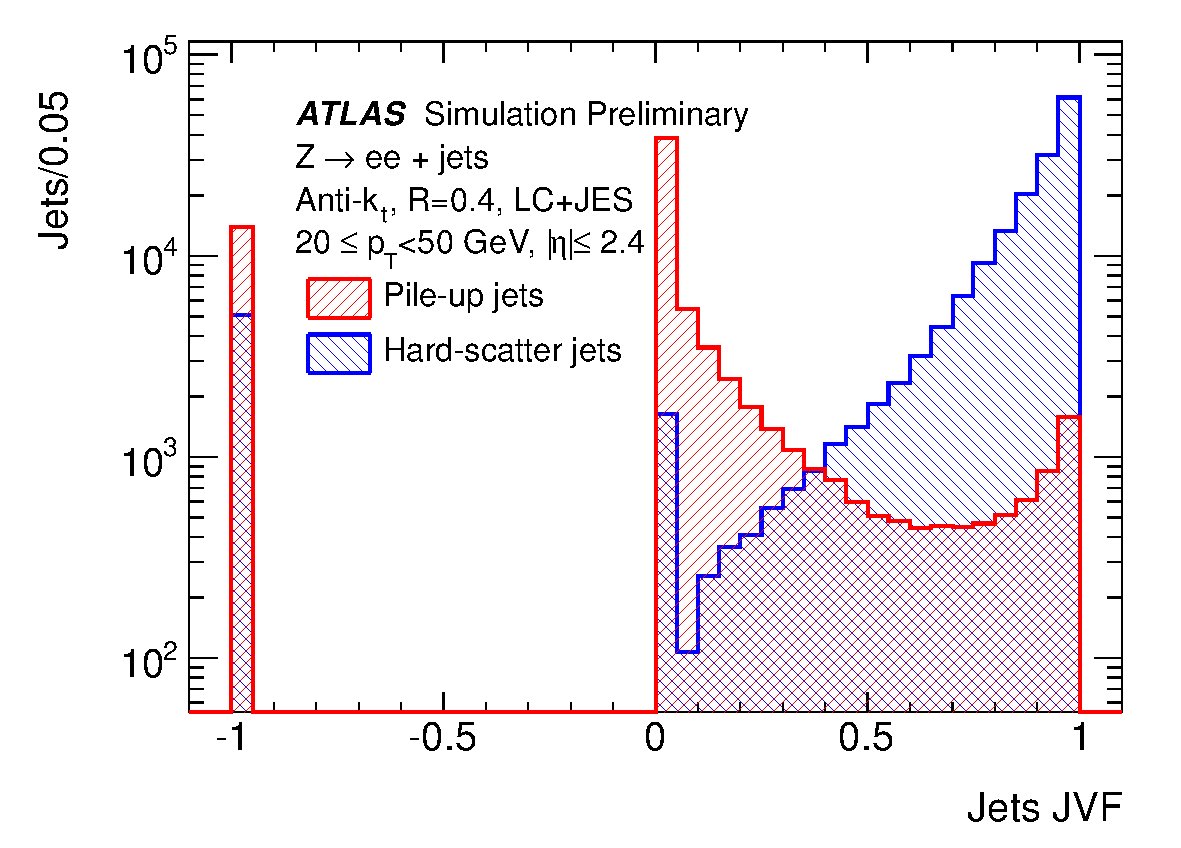
\includegraphics[width=0.6\textwidth]{fig/reconstruction/JVF_plot.pdf}
    \caption[]{Distribution of JVF for HS (blue) and pileup (red) jets
    with $20\gev<\pt<50\gev$ and $|\eta| < 2.5$ in simulated \zjets events.~\cite{bib:ATLAS-CONF-2013-083}}
\label{chap:reconstruction:fig:jvf}
\end{figure}

The discriminating power of JVF is illustrated in
figure~\ref{chap:reconstruction:fig:jvf}, where the JVF distributions
for HS and pileup jets are shown for \zjets simulation. 






\section{Missing Transverse Energy}
\label{chap:reco:sec:met}

Many physics analyses seek final states with particles that are weakly
interacting and just pass through the detector undetected. Because the
initial momenta of the incoming partons is approximately zero in the
transverse plane, the presence of these undetected particles can be
inferred by measuring the missing momentum in this
direction. Mathematically, this is seen by requiring momentum conservation

\begin{equation}
\begin{aligned}
\vect{p}^{\textrm{incoming}}_{\textrm{T}} = 0 &=
\vect{p}^{\textrm{outgoing}}_{\textrm{T}} \\
&= \vect{p}^{\textrm{visible}}_{\textrm{T}} +
\vect{p}^{\textrm{missing}}_{\textrm{T}}, 
\end{aligned}
\end{equation}

\noindent
which implies that $\vect{p}^{\textrm{missing}}_{\textrm{T}}$ is
obtained by measuring
$-\vect{p}^{\textrm{visible}}_{\textrm{T}}$. Since the longitudinal momenta of the
incoming partons is not known, this quantity can not be inferred
through momentum conservation, making it impossible to reconstruct the
4-momentum of the undetected particles. In this thesis, the missing transverse
momentum of the visible particles
$\vect{p}^{\textrm{visible}}_{\textrm{T}}$ is reconstructed using
either calorimeter deposits or tracks. The former is denoted \calomet
while the latter is denoted \trkmet. Generically, missing transverse
energy will be referred to as \etmiss.

\subsection{Calorimeter \etmiss Reconstruction}

Calorimeter-based missing transverse energy uses information from the
calorimeter as well as the tracking systems for muons, and can
therefore be decomposed into two terms~\cite{bib:ATLAS-CONF-2013-082}. The calorimeter term is
further decomposed into the high-\pt~ physics objects which are
reconstructed from calorimeter information, as well as a soft term for
the low energy deposits not associated to a high-\pt object:

\begin{equation}
\vect{\ensuremath{E}}_{\mathrm{T}}^{\mathrm{miss, CALO}} =
\vect{\ensuremath{E}}_{\mathrm{T}}^{\mathrm{miss},e} +
\vect{\ensuremath{E}}_{\mathrm{T}}^{\mathrm{miss},\gamma} +
\vect{\ensuremath{E}}_{\mathrm{T}}^{\mathrm{miss},\tau} +
\vect{\ensuremath{E}}_{\mathrm{T}}^{\mathrm{miss,jets}} +
\vect{\ensuremath{E}}_{\mathrm{T}}^{\mathrm{miss,soft}} + 
\vect{\ensuremath{E}}_{\mathrm{T}}^{\mathrm{miss},\mu}
\label{chap:reco:equation:etmiss}
\end{equation}

\noindent
To avoid double-counting energy in the calorimeter, selection of the
objects going into equation~\ref{chap:reco:equation:etmiss} is done
sequentially. First, the
$\vect{\ensuremath{E}}_{\mathrm{T}}^{\mathrm{miss},e}$ term is defined
using reconstructed electrons (section~\ref{chap:reco:sec:electron})
with $\pt > 10 \gev$ (what kind of electrons?). Then photons with $\pt
> 10 \gev$ and without any overlap with reconstructed electrons are
selected. High-\pt~jets ($\pt > 20 \gev$) are reconstructed with
topological clusters using the \antikt algorithm with distance measure
$R=0.4$ (section~\ref{chap:reco:sec:jet}). These clusters are required
to be isolated from those associated to electrons or photons. To reject jets from
pile-up, jets with $|\eta| < 2.4$ and $20~\gev < \pt < 50~\gev$ are
required to have $|\textrm{JVF}| > 0$
(section~\ref{chap:reco:sec:jet:subsec:quality}) (I don't think this
is the case for METRefFinal). The final calorimeter term represents
energy in the event that is not associated with high-\pt~objects. This
soft term is built from LCW-calibrated topological clusters which do
not have an explicit $E_T$ requirement but are robust against
electronic and pileup noise
(section~\ref{chap:reco:sec:cluster}. Given that it is not possible to
reliably match a cluster to a primary vertex, the soft term is highly sensitive
to in-time pileup, as shown in
figure~\ref{chap:reconstruction:fig:softterm_pileup}. In an inclusive
$Z\rightarrow{\mu\mu}$ sample, the average soft term at $\nvtx = 1$ is
around $10 \gev$ and increases to $40 \gev$ at $\nvtx = 25$. This
term significantly degrades both the magnitude and direction
resolutions for \etmiss. Various corrections which help to mitigate
the dependence on pileup have been used in
ATLAS~\cite{bib:ATLAS-CONF-2014-019}, but for the analysis presented
in this thesis, the baseline calorimeter \etmiss definition without
corrections is used. 

\begin{figure}[h]
    \centering
    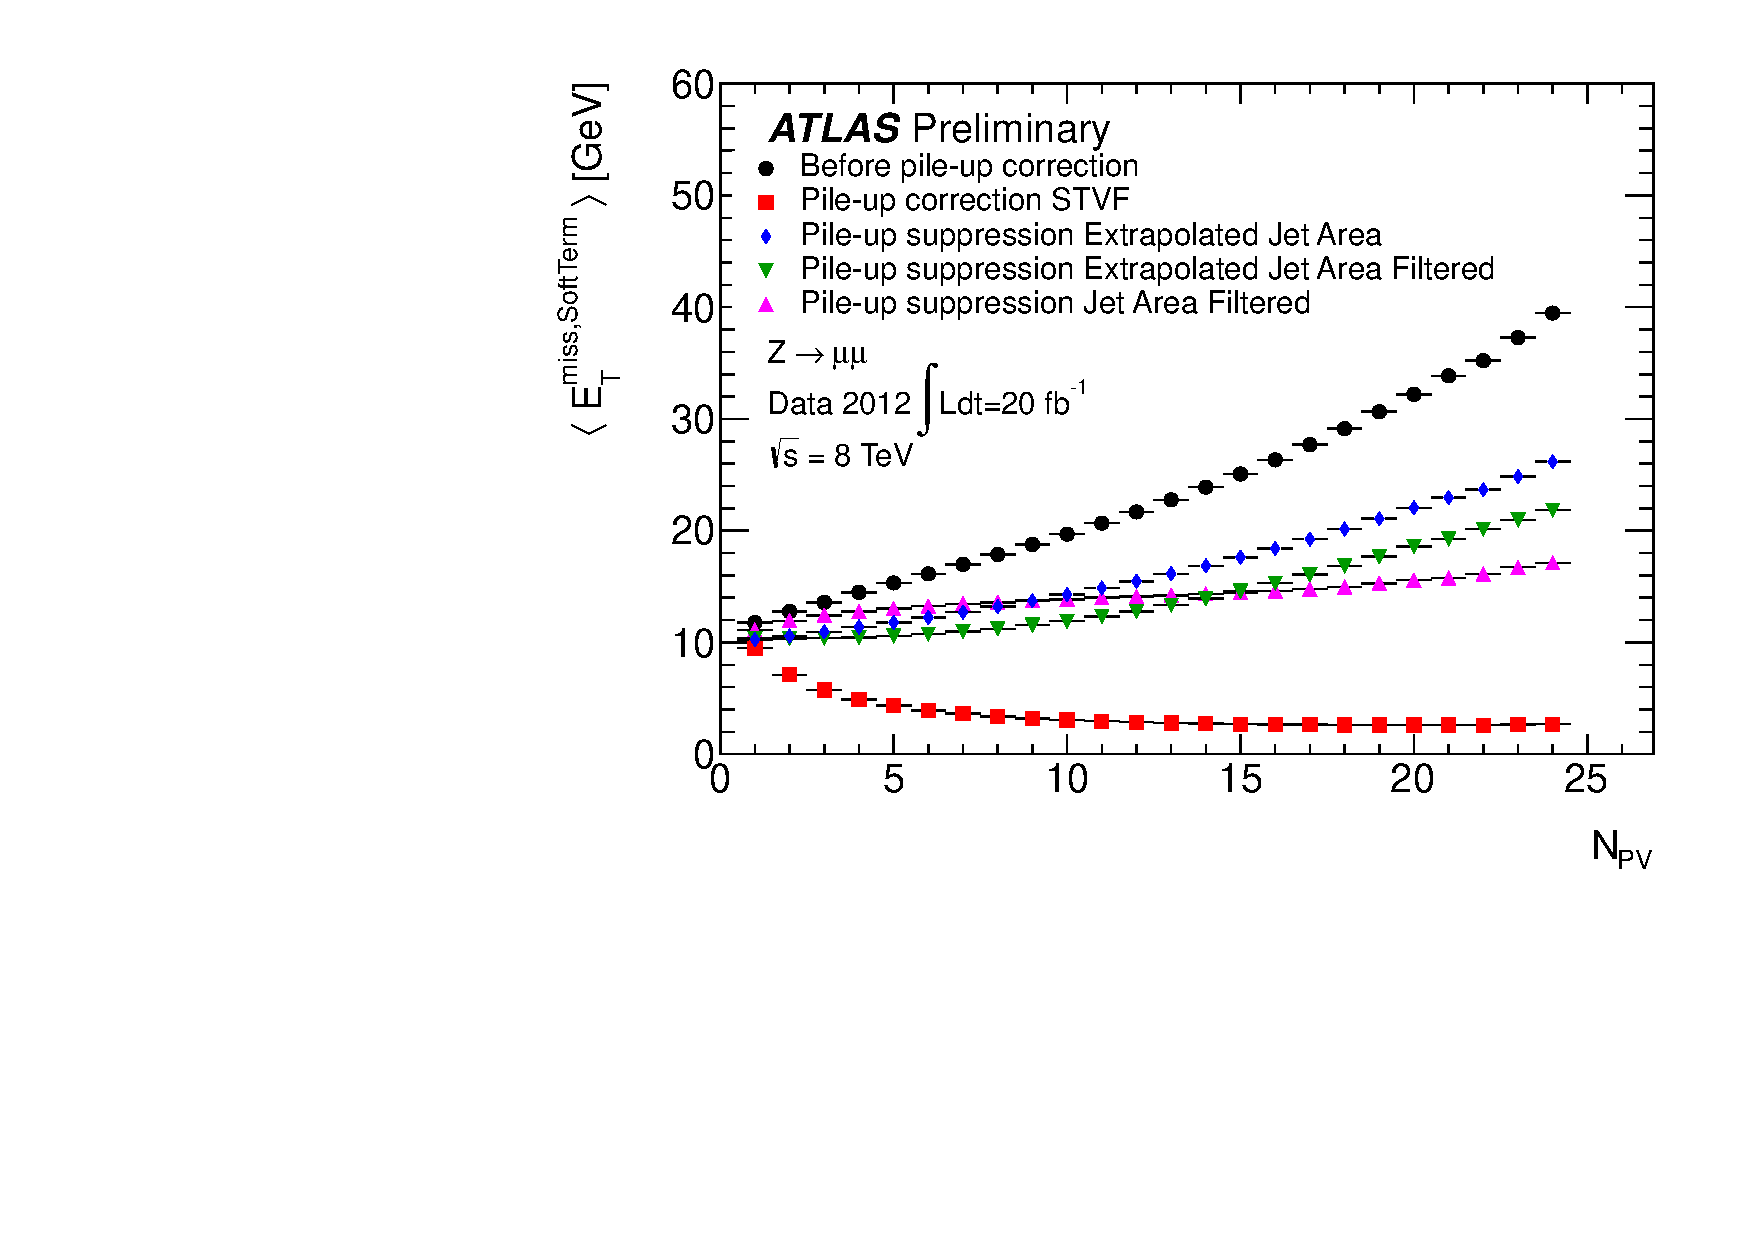
\includegraphics[width=0.6\textwidth]{fig/reconstruction/cell_out_PU_Zmumu.pdf}
    \caption[]{The average calorimeter \etmiss soft term $\left \langle
      E_{\mathrm{T}}^{\mathrm{miss,soft}} \right \rangle$ (shown in black) as a
      function of the number of primary vertices for an inclusive $Z\rightarrow{\mu\mu}$
      sample in $\sqrts=8 \tev$ data~\cite{bib:ATLAS-CONF-2014-019}.}
\label{chap:reconstruction:fig:softterm_pileup}
\end{figure}

For the
muon term, combined muons (section~\ref{chap:reco:sec:muon}) with $\pt
> 6~\gev$ are used
where there is both ID and MS coverage ($0.1 < |\eta| < 2.5$). Because
muons usually leave energy clusters in the calorimeter, and the
combined muon fit accounts for this loss, the combined muon energy is
double-counted. This is corrected by subtracting the parameterized energy loss in the
calorimeter from the fitted muon momentum. Outside of the ID,
standalone muons are used, while in regions with limited MS coverage
($|\eta| < 0.1$), ID track muons are used.

\subsection{Track \etmiss Reconstruction}

As mentioned in the previous section, \calomet is sensitive to in-time
pileup, degrading its resolution for large \nvtx events. Track \etmiss
seeks to suppress pileup dependence by replacing the clusters defining
the soft term with tracks matched to the primary vertex of the
event (section~\ref{chap:reco:sec:tracks}. These tracks are required
to have $\pt > 500 \mev$ and $|\eta| < 2.5$, with additional quality
requirements: $|d_0 < 1.5$~mm, $|z_0\sin(\theta) < 1.5$~mm,
$N_{\textrm{hits}}^{\textrm{pixel}} \geq 1$, and
$N_{\textrm{hits}}^{\textrm{SCT}} \geq 6$. If a track fails these
quality criteria, but pass requirements associated with electrons and
muons, then the associated leptons \pt~replaces the track. The lepton
requirements are similar to those in the \calomet definition, with
some important exceptions which will be discussed in
chapter~\ref{chap:analysis}. Moreover, tracks that fall within a cone
of $R=0.4$ of a jet are not included in \etmiss; instead the jet
itself is used. The rationale is that
if tracks are used to define \etmiss instead of reconstructed jets,
neutral tracks associated with the jets are missed, thereby degrading
the \etmiss resolution. The specific definition of a jet is
analysis-dependent, and will therefore be described in detail in
chapter~\ref{chap:analysis}. 

